\PassOptionsToPackage{unicode=true}{hyperref} % options for packages loaded elsewhere
\PassOptionsToPackage{hyphens}{url}
\PassOptionsToPackage{dvipsnames,svgnames*,x11names*}{xcolor}
%
\documentclass[ignorenonframetext,aspectratio=169]{beamer}
\usepackage{pgfpages}
\setbeamertemplate{caption}[numbered]
\setbeamertemplate{caption label separator}{: }
\setbeamercolor{caption name}{fg=normal text.fg}
\beamertemplatenavigationsymbolsempty
% Prevent slide breaks in the middle of a paragraph:
\widowpenalties 1 10000
\raggedbottom
\setbeamertemplate{part page}{
\centering
\begin{beamercolorbox}[sep=16pt,center]{part title}
  \usebeamerfont{part title}\insertpart\par
\end{beamercolorbox}
}
\setbeamertemplate{section page}{
\centering
\begin{beamercolorbox}[sep=12pt,center]{part title}
  \usebeamerfont{section title}\insertsection\par
\end{beamercolorbox}
}
\setbeamertemplate{subsection page}{
\centering
\begin{beamercolorbox}[sep=8pt,center]{part title}
  \usebeamerfont{subsection title}\insertsubsection\par
\end{beamercolorbox}
}
\AtBeginPart{
  \frame{\partpage}
}
\AtBeginSection{
  \ifbibliography
  \else
    \frame{\sectionpage}
  \fi
}
\AtBeginSubsection{
  \frame{\subsectionpage}
}
\usepackage{lmodern}
\usepackage{amssymb,amsmath}
\usepackage{ifxetex,ifluatex}
\usepackage{fixltx2e} % provides \textsubscript
\ifnum 0\ifxetex 1\fi\ifluatex 1\fi=0 % if pdftex
  \usepackage[T1]{fontenc}
  \usepackage[utf8]{inputenc}
  \usepackage{textcomp} % provides euro and other symbols
\else % if luatex or xelatex
  \usepackage{unicode-math}
  \defaultfontfeatures{Ligatures=TeX,Scale=MatchLowercase}
\fi
\usetheme[]{AnnArbor}
\usecolortheme{dolphin}
\usefonttheme{structuresmallcapsserif}
% use upquote if available, for straight quotes in verbatim environments
\IfFileExists{upquote.sty}{\usepackage{upquote}}{}
% use microtype if available
\IfFileExists{microtype.sty}{%
\usepackage[]{microtype}
\UseMicrotypeSet[protrusion]{basicmath} % disable protrusion for tt fonts
}{}
\IfFileExists{parskip.sty}{%
\usepackage{parskip}
}{% else
\setlength{\parindent}{0pt}
\setlength{\parskip}{6pt plus 2pt minus 1pt}
}
\usepackage{xcolor}
\usepackage{hyperref}
\hypersetup{
            pdftitle={Gene transfer in bacteria},
            pdfauthor={Deependra Dhakal},
            colorlinks=true,
            linkcolor=red,
            filecolor=Maroon,
            citecolor=blue,
            urlcolor=red,
            breaklinks=true}
\urlstyle{same}  % don't use monospace font for urls
\newif\ifbibliography
\setlength{\emergencystretch}{3em}  % prevent overfull lines
\providecommand{\tightlist}{%
  \setlength{\itemsep}{0pt}\setlength{\parskip}{0pt}}
\setcounter{secnumdepth}{0}

% set default figure placement to htbp
\makeatletter
\def\fps@figure{htbp}
\makeatother

\usepackage{tikz}
\usepackage[absolute,overlay]{textpos}
\usepackage{booktabs}
\usepackage{longtable}
\usepackage{array}
\usepackage{multirow}
\usepackage{wrapfig}
\usepackage{float}
\usepackage{colortbl}
\usepackage{pdflscape}
\usepackage{tabu}
\usepackage{threeparttable}
\usepackage{threeparttablex}
\usepackage[normalem]{ulem}
\usepackage{makecell}
\usepackage{xcolor}

% define new footline defination
\setbeamertemplate{footline}
{
    \leavevmode%
    \hbox{%
        \begin{beamercolorbox}[wd = .5\paperwidth, ht = 1ex, dp = 1ex, center]{author in head/foot}%
            Text in footer
        \end{beamercolorbox}%
        \begin{beamercolorbox}[wd = .5\paperwidth, ht = 1ex, dp = 1ex, center]{date in head/foot}%
            \insertframenumber{}
        \end{beamercolorbox}
    }%
    \vskip3pt%
}
% add footline defination to the beamer template
\addtobeamertemplate{footline}{\begin{center}\rule{0.6\paperwidth}{0.4pt}\end{center}\vspace*{-1ex}}{}

% % set titlepage in a TikZ node for modifications
\setbeamertemplate{title page}{
\tikz\node[opacity=0.3] {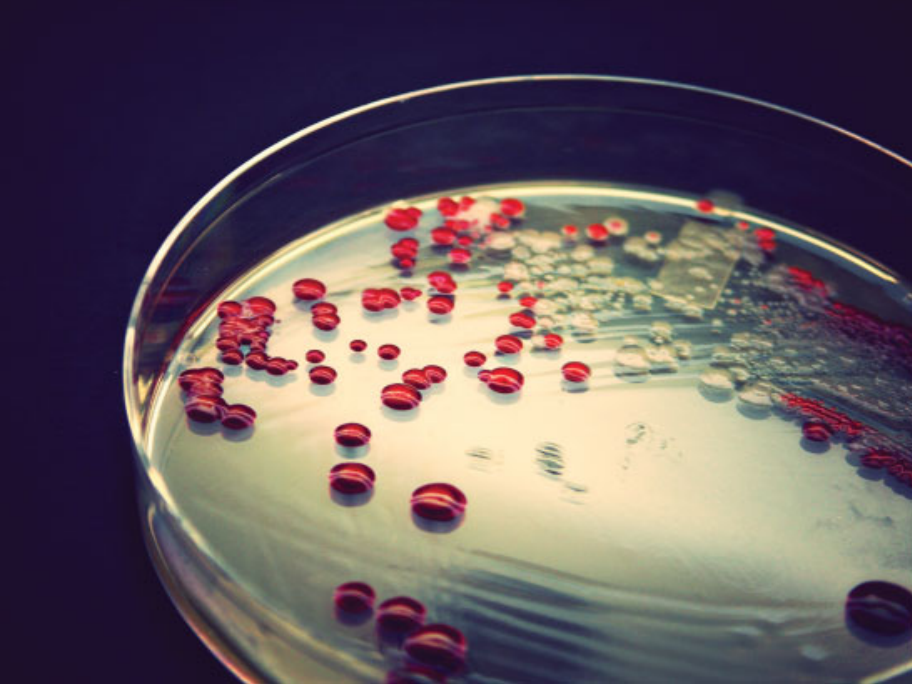
\includegraphics[height=\paperheight,width=\paperwidth]{03-gene_transfer_in_bacteria_bacterial_colony.png}};
% \tikz\node[opacity=0.8] {\includegraphics[width=5cm,ext=.1-overview_mutation_cover.png,type=png,read=.1-overview_mutation_cover.png]{1}} % if name shall contain dots, suppose filename = 01.1-overview_mutation_cover.png
\begin{textblock}{15}(1.5,2.8)\usebeamerfont{title} % 1.5 is x position in page
{\color{white}\raggedright\par\inserttitle}
\end{textblock}
\begin{textblock}{7.5}(1.5,7) % 1.5 is x position in page
{\color{white}\raggedright{\insertauthor}\mbox{}\\[0.2cm]
\insertdate}
\end{textblock}} % dd_rookie modified, figure is top aligned


% % set caption font size
% % note that beamer presentation native captions have their own configs
% \usepackage{caption}
% \captionsetup{font=footnotesize}

% this font option is amenable for beamer
\setbeamerfont{caption}{size=\tiny}

% some beamer themes naturally might not support navigation symbols
% \setbeamertemplate{navigation symbols}{} % remove navigation symbols

\setbeamertemplate{footline}[page number] % insert page number in footline

% \setbeamertemplate{navigation symbols}{slide} % insert slide indication in navigation
% \setbeamertemplate{navigation symbols}{frame} % insert frame indication in navigation
% \setbeamertemplate{navigation symbols}{section} % insert section indication in navigation
% \setbeamertemplate{navigation symbols}{subsection} % insert subsection indication in navigation

% \AtBeginSubsection{} % supress subsection display

\title{Gene transfer in bacteria}
\author{Deependra Dhakal}
\providecommand{\institute}[1]{}
\institute{GAASC, Baitadi \and Tribhuwan University}
\date{Academic year 2019-2020}

\begin{document}
\frame{\titlepage}

\begin{frame}
\tableofcontents[hideallsubsections]
\end{frame}
\hypertarget{bacterial-genetics}{%
\section{Bacterial genetics}\label{bacterial-genetics}}

\begin{frame}{Features of prokaryotic and eukaryotic cells}
\protect\hypertarget{features-of-prokaryotic-and-eukaryotic-cells}{}

\begin{itemize}
\tightlist
\item
  A eukaryotic cell is subdivided by internal membranes into various
  membrane-enclosed organelles (Figure \ref{fig:eu-prokaryotic-cell}).
\item
  In eukaryotic cells, nucleus contains the cell's DNA.
\item
  The other organelles are located in the cytoplasm, the entire region
  between the nucleus and outer membrane of the cell.
\item
  The chloroplast is a characterstic organelle found in eukaryotic cells
  that carry out photosynthesis.
\item
  Prokaryotic cells are much simpler and generally smaller than
  eukaryotic cells.
\item
  In a prokaryotic cell, the DNA is not separated from the rest of the
  cell by enclosure in a membrane-bounded nucleus.
\item
  Prokaryotic cells also lack the other kinds of membrane-enclosed
  organelles.
\end{itemize}

\end{frame}

\begin{frame}{Features of prokaryotic and eukaryotic cells}
\protect\hypertarget{features-of-prokaryotic-and-eukaryotic-cells-1}{}

\begin{figure}
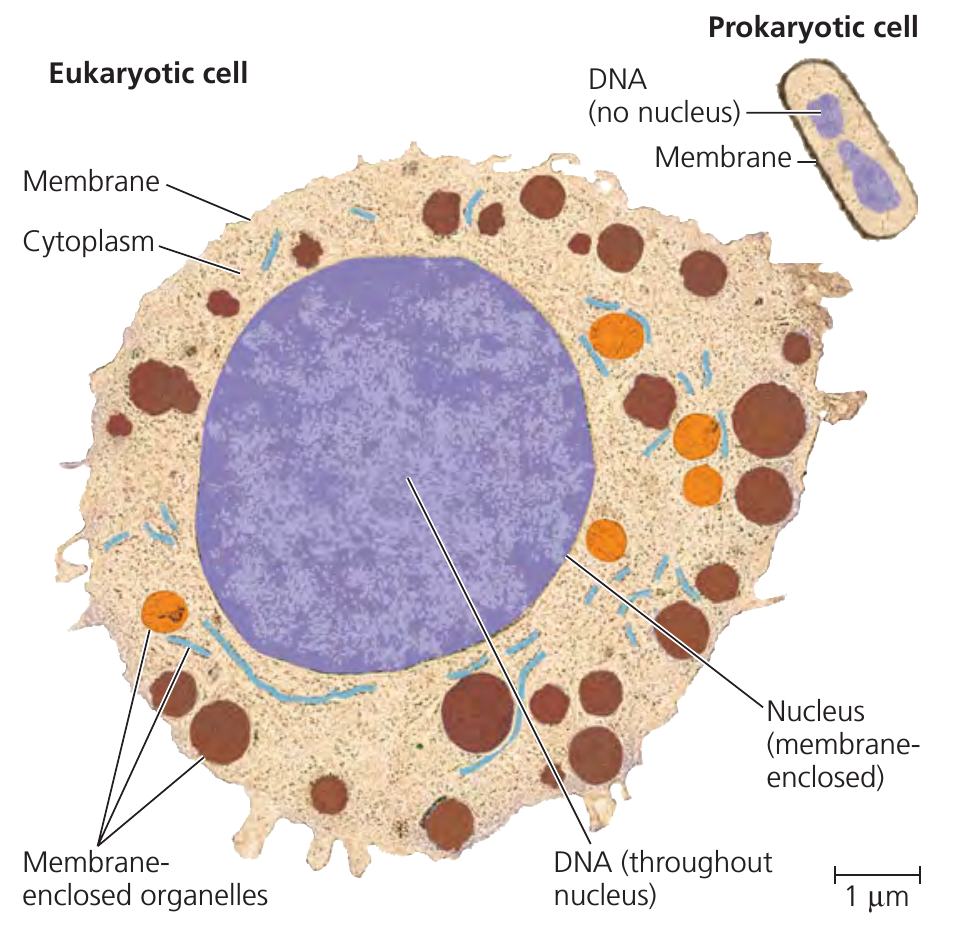
\includegraphics[width=0.35\linewidth]{./../images/eukaryotic_prokaryotic} \caption{Contrasting eukaryotic and prokaryotic cells in size and complexity.}\label{fig:eu-prokaryotic-cell}
\end{figure}

\end{frame}

\begin{frame}{Features of prokaryotic and eukaryotic cells}
\protect\hypertarget{features-of-prokaryotic-and-eukaryotic-cells-2}{}

\begin{table}[t]

\caption{\label{tab:eu-arch-prokaryotic-cell}Comparison of some lower life forms}
\centering
\fontsize{6}{8}\selectfont
\begin{tabular}{>{\raggedright\arraybackslash}p{15em}>{\raggedright\arraybackslash}p{15em}>{\raggedright\arraybackslash}p{15em}l}
\toprule
  & Bacteria & Archaea & Eukarya\\
\midrule
\rowcolor{gray!6}  Nuclear envelope & Absent & Absent & Present\\
Membrane enclosed organelles & Absent & Absent & Present\\
\rowcolor{gray!6}  Peptidoglycan in cell wall & Present & Absent & Absent\\
Membrane lipids & Unbranched hydrocarbons & Some branched hydrocarbons & Unbranched hydrocarbons\\
\rowcolor{gray!6}  RNA polymerase & One kind & Several kinds & Several kinds\\
\addlinespace
Initiator amino acid for protein synthesis & Formyl-methionine & Methionine & Methionine\\
\rowcolor{gray!6}  Introns in genes & Very rare & Present in some genes & Present in many genes\\
Response to the antibiotics Streptomycin and chlormaphenicol & Growth inhibited & Growth not inhibited & Growth not inhibited\\
\rowcolor{gray!6}  Histones associated with DNA & Absent & Present in some species & Present\\
Circular chromosome & Present & Present & Absent\\
\addlinespace
\rowcolor{gray!6}  Growth at temperatures greater than 100 degree C & No & Some species & No\\
\bottomrule
\end{tabular}
\end{table}

\end{frame}

\begin{frame}{DNA and chromosome structure}
\protect\hypertarget{dna-and-chromosome-structure}{}

\begin{figure}
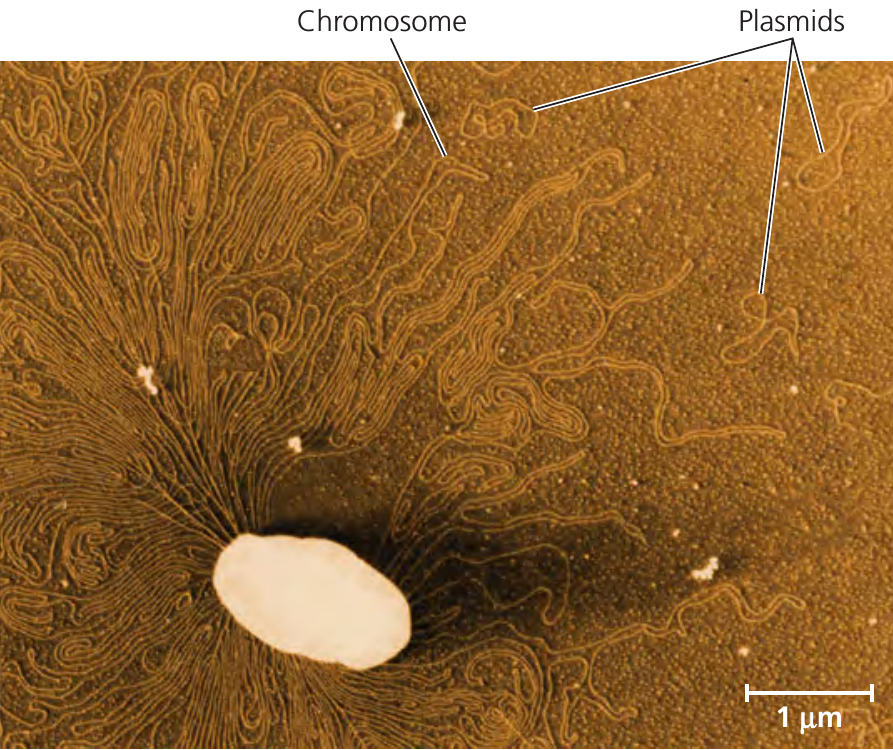
\includegraphics[width=0.38\linewidth]{./../images/prokaryotic_chr_plasmid} \caption{A prokaryotic chromosome and plasmids. The thin, tangled loops surrounding this ruptured E. coli cell are parts of the cell’s large, circular chromosome (colorized TEM). Three of the cell’s plasmids, the much smaller rings of DNA, are also shown.}\label{fig:prokaryotic-dna}
\end{figure}

\end{frame}

\hypertarget{major-genetic-material-transfer-processes}{%
\section{Major genetic material transfer
processes}\label{major-genetic-material-transfer-processes}}

\begin{frame}{Genetic transformation}
\protect\hypertarget{genetic-transformation}{}

\begin{itemize}
\tightlist
\item
  First observed in bacteria and first bacterial system for genetic
  transfer to be discovered.
\item
  Naturally occurs in only certain bacteria, but under laboratory
  conditions it seems to be possible with any cell type, prokaryotic or
  eukaryotic.
\item
  When a bacterial cell (living or dead) releases some DNA into the
  surrounding medium, this DNA is, of course, vulnerable to degradation
  but may encounter another bacterial cell before any significant change
  can occur.
\end{itemize}

\end{frame}

\begin{frame}{Genetic transformation}
\protect\hypertarget{genetic-transformation-1}{}

\begin{itemize}
\tightlist
\item
  The second cell may take up the DNA, transport it across the cell wall
  and cell membrane, and allow it to recombine with the homologous
  portion of the resident bacterial chromosome.
\item
  The resulting recombinant cell is called a transformant.
\item
  The amount of DNA transferred per event is small, on the order of 10
  kb in length.
\end{itemize}

\end{frame}

\begin{frame}{Transformation}
\protect\hypertarget{transformation}{}

\begin{figure}
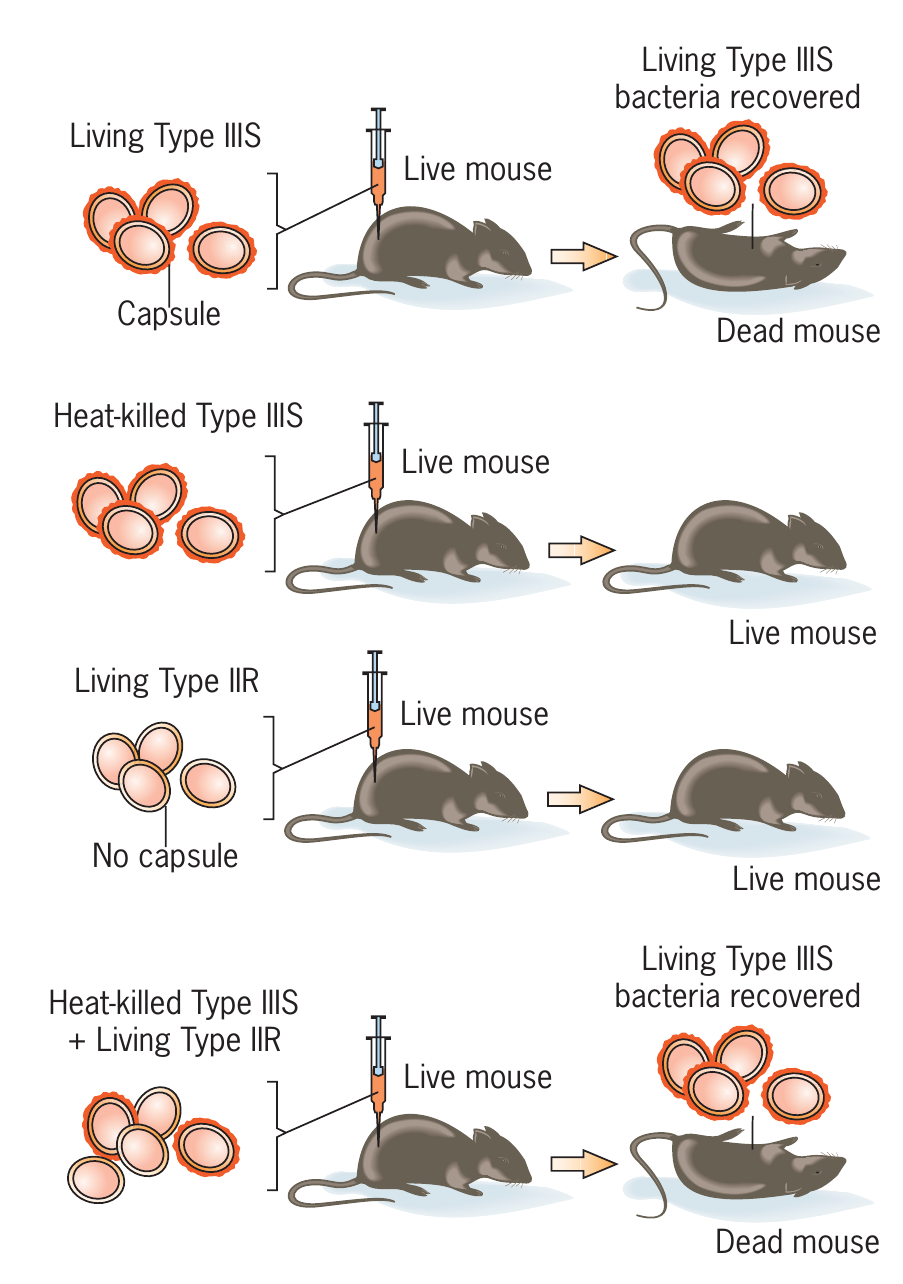
\includegraphics[width=0.25\linewidth]{./../images/bacterial_transformation} \caption{Griffith's discovery of transformation in Streptococcus pneumoniae}\label{fig:transformation-griffith}
\end{figure}

\end{frame}

\begin{frame}{Transduction}
\protect\hypertarget{transduction}{}

\begin{itemize}
\tightlist
\item
  Bacterial virus (bacteriophage) is intimately involved in the genetic
  transfer process.
\item
  Phage infections begin with adsorption of virus particles to specific
  receptor sites on the host cell surface. The nucleic acid contained
  inside the viral protein coat is then transferred to the cytoplasm of
  the bacterial cell, where it becomes metabolically active and
  undergoes replication and transcription.
\item
  Typically there are two possible outcomes of phage infection.
\end{itemize}

\end{frame}

\begin{frame}{Transduction}
\protect\hypertarget{transduction-1}{}

\begin{itemize}
\tightlist
\item
  During a \textbf{lytic response}, the virus produces structural
  components of new phage particles, packages its nucleic acid inside
  them, and then causes the cell to lyse and release progeny phage.
\item
  During a \textbf{temperate response}, the virus establishes a stable
  relationship with a host cell in which some phage functions are
  expressed, but not those that lead to uncontrolled DNA replication or
  the production and assembly of new particles.
\end{itemize}

\end{frame}

\begin{frame}{Transduction: responses}
\protect\hypertarget{transduction-responses}{}

\begin{figure}
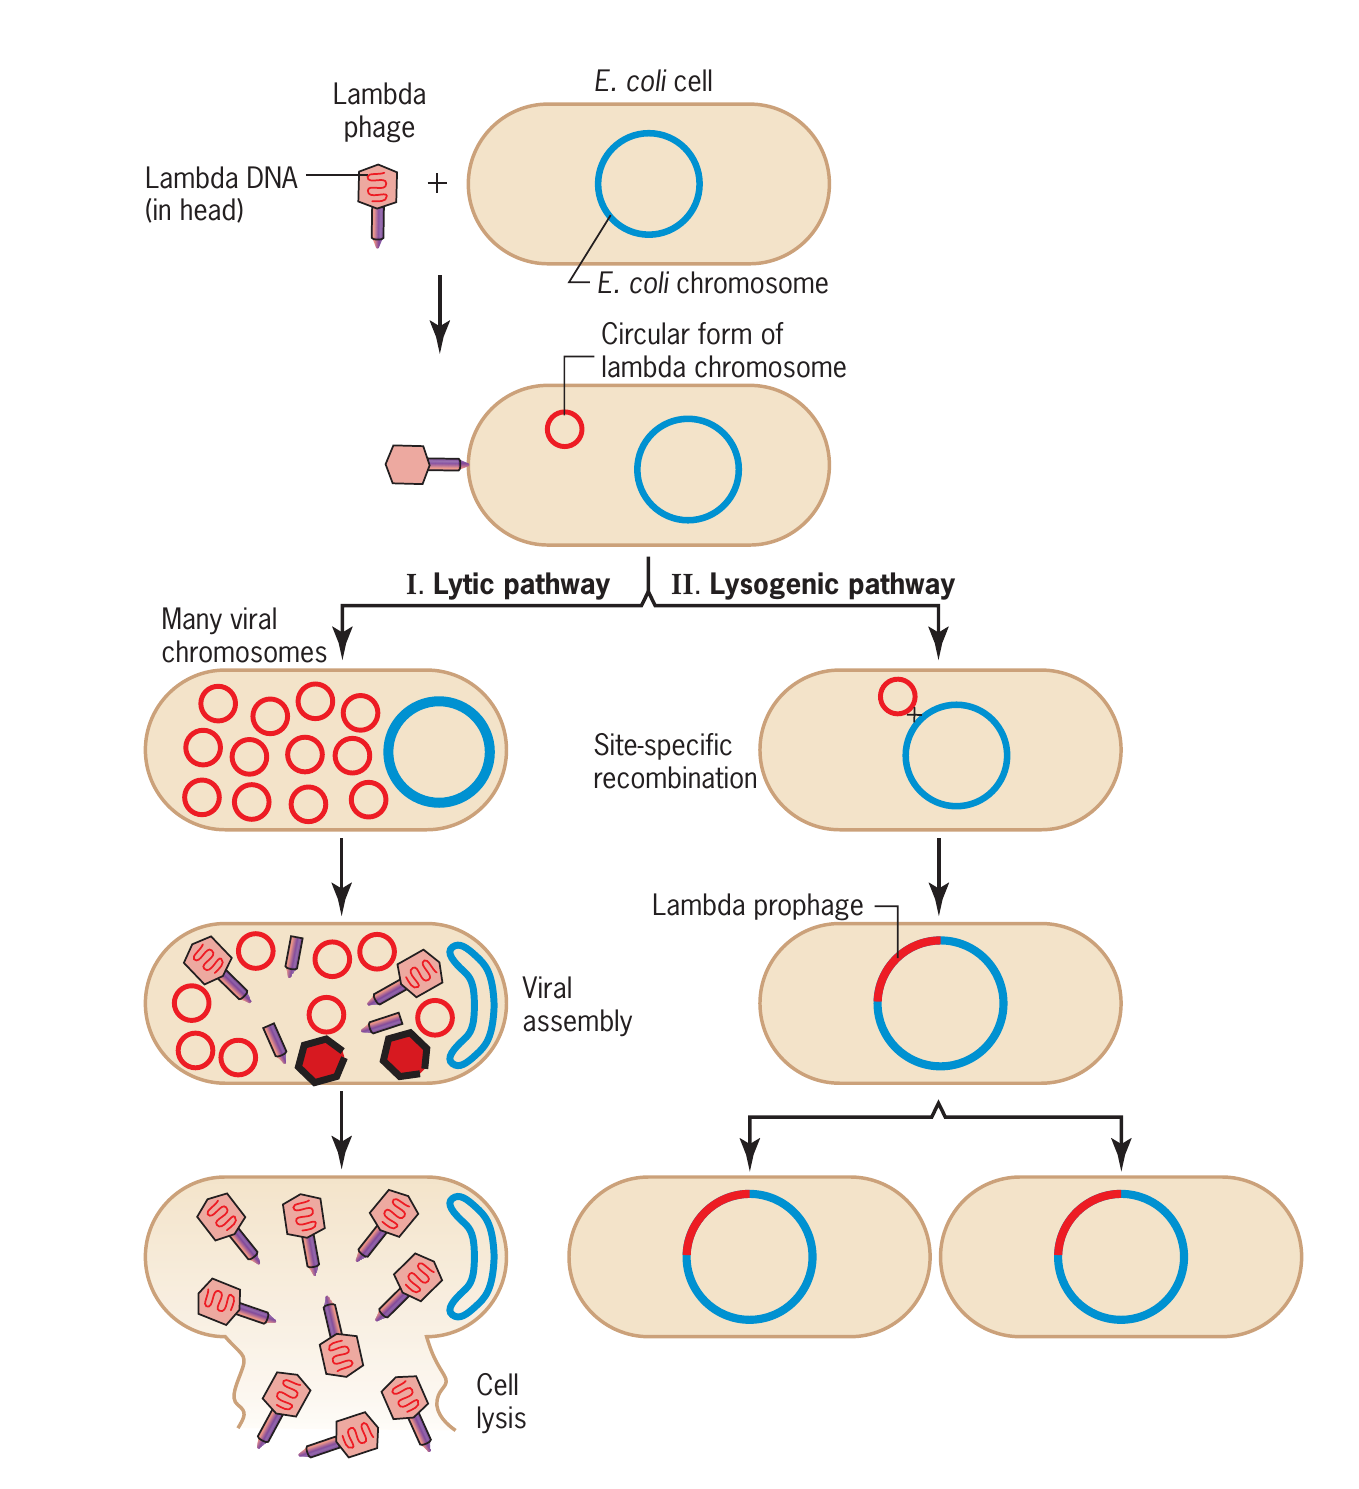
\includegraphics[width=0.25\linewidth]{./../images/bacteriophage_stages} \caption{The life cycle of bacteriophage $\lambda$. The two intracellular states of bacteriophage lambda: lytic growth and lysogeny. Lambda is smaller than T4; however, its life cycle is more complex. Note, bacteriophage T4 is a lytic phage; when it infects a bacterium, it replicates and kills the host}\label{fig:transduction-bacteriophage}
\end{figure}

\end{frame}

\begin{frame}{Transduction}
\protect\hypertarget{transduction-2}{}

\begin{itemize}
\tightlist
\item
  Instead, viral DNA is replicated along with host DNA, usually as an
  integral part of the same molecule, and is transmitted to all progeny
  cells.
\item
  Occasionally \textbf{lysogens} (cells carrying a temperate phage)
  undergo a metabolic shift that reactivates the viral DNA. The result
  is the same as for an initial lytic response. - Some phages may give
  only lytic responses and some only temperate ones; some, however, may
  give either response, depending on growth conditions.
\end{itemize}

\end{frame}

\begin{frame}{Transduction: Transducing bacterial cell}
\protect\hypertarget{transduction-transducing-bacterial-cell}{}

\begin{itemize}
\tightlist
\item
  During the course of a phage infection of a bacterial cell, some or
  all of the viral DNA inside an individual virion (virus particle) may
  be replaced by bacterial DNA, and this process may occur only rarely
  or with great frequency.
\item
  After such an altered phage particle is released into the medium, it
  may encounter another bacterial cell and attempt to initiate an
  infection. In so doing, however, it transfers the DNA fragment from
  the previous host's chromosome.
\item
  If the newly infected cells are not killed and the DNA fragment can
  either replicate or recombine, the result is the production of
  \textbf{transductants}.
\end{itemize}

\end{frame}

\begin{frame}{Transduction: Amount of change}
\protect\hypertarget{transduction-amount-of-change}{}

\begin{itemize}
\tightlist
\item
  The amount of DNA transferred by these means varies considerably, but
  generally is not more than the amount of DNA normally present in a
  single bacteriophage particle (\textasciitilde{}200 kbp).
\item
  The actual amount of DNA recombined is significantly less in most
  cases and, in addition, depends on whether the transduction is
  generalized or specialized.
\end{itemize}

\end{frame}

\begin{frame}{Transduction: Generalized and specialized}
\protect\hypertarget{transduction-generalized-and-specialized}{}

\begin{itemize}
\tightlist
\item
  During \textbf{generalized transduction} the phage enzyme system that
  packages viral DNA attaches to the bacterial chromosome and packages
  some of that DNA instead. The DNA that is packaged is chosen on a more
  or less random basis, and as a result it is possible for any piece of
  host genetic information to be transferred.
\item
  \textbf{Specialized transduction} involves a temperate phage that has
  physically integrated its DNA into the bacterial chromosome at a
  specific site. As mentioned earlier, such an integrated phage may be
  stable for long periods of time.
\end{itemize}

\end{frame}

\begin{frame}{Transduction: Generalized and specialized}
\protect\hypertarget{transduction-generalized-and-specialized-1}{}

\begin{itemize}
\tightlist
\item
  However, it may reactivate and replicate itself independent of the
  bacterial chromosome. During the reactivation process, it is possible
  for a mistake to occur so that some bacterial DNA located adjacent to
  one end of the viral DNA is also excised from the chromosome instead
  of the appropriate DNA from the other end of the viral genome.
\item
  Because the overall size of the excised DNA must be nearly constant,
  only certain pieces of genetic information can be transferred, and
  their size depends on the physical nature of the mistake that caused
  their production.
\end{itemize}

\end{frame}

\begin{frame}{Transduction: Generalized}
\protect\hypertarget{transduction-generalized}{}

\begin{figure}
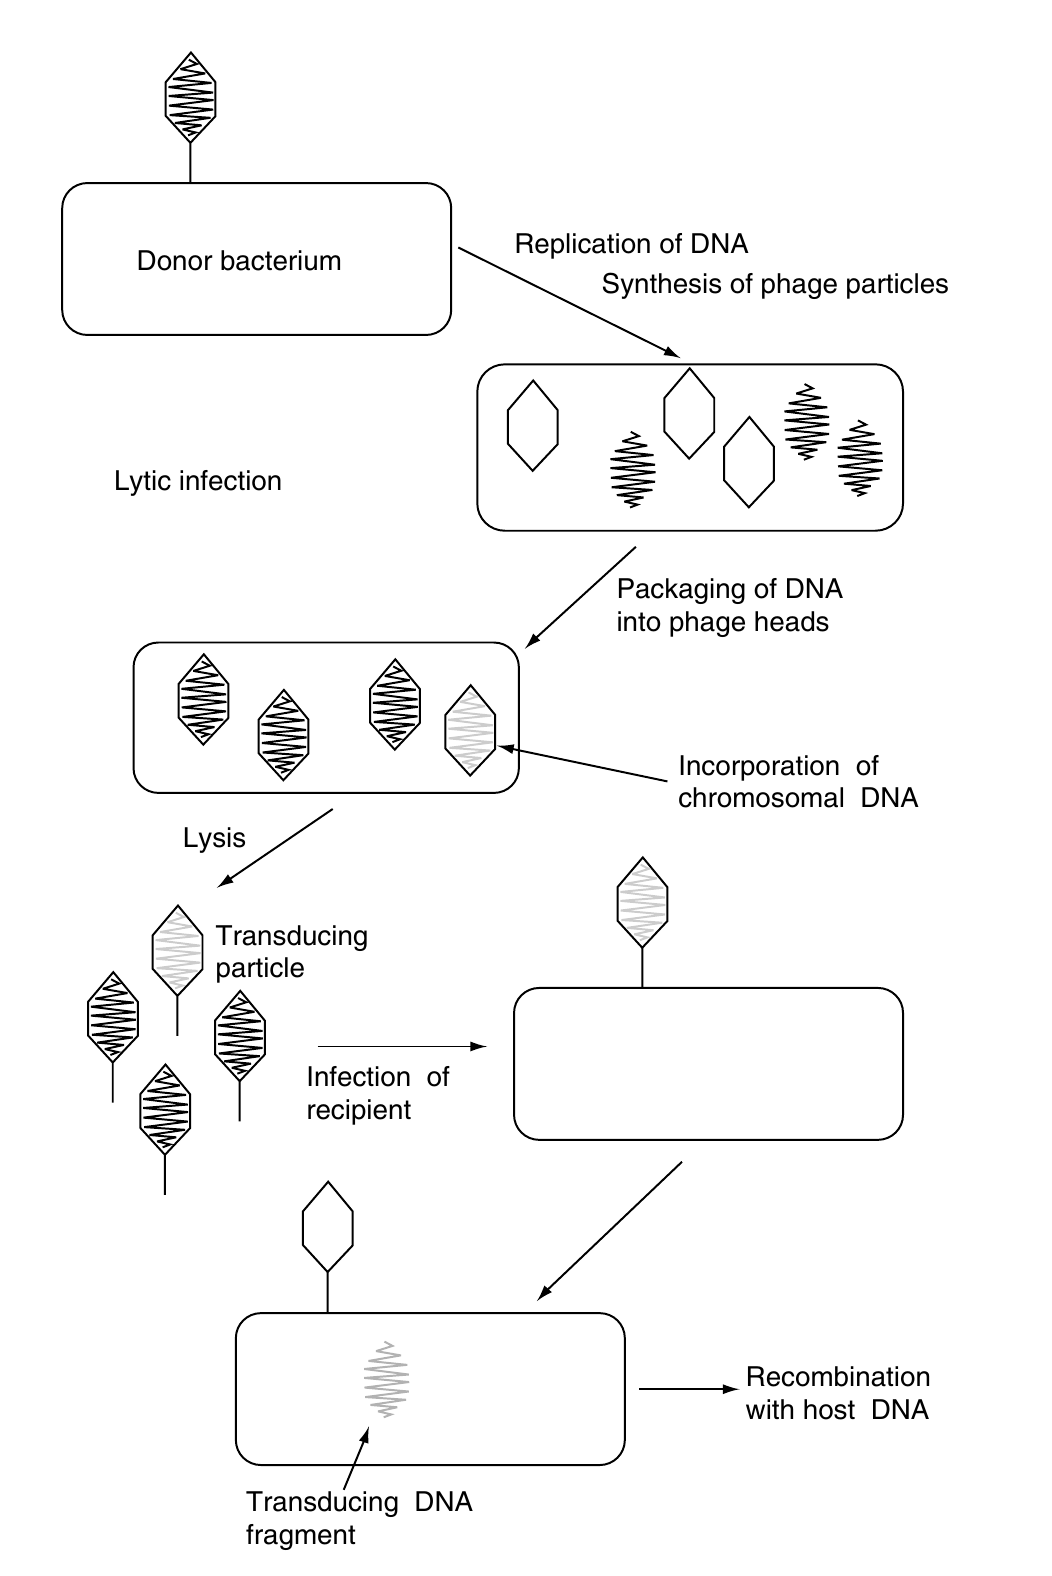
\includegraphics[width=0.25\linewidth]{./../images/transduction_generalized} \caption{Generalized transduction}\label{fig:transduction-gen}
\end{figure}

\end{frame}

\begin{frame}{Conjugation}
\protect\hypertarget{conjugation}{}

\begin{itemize}
\tightlist
\item
  In yeast the result of conjugation is fusion of haploid cells and
  formation of a diploid cell type.
\item
  In a bacterium such as E. coli, instead of cell fusion there is
  unidirectional transfer of DNA from a donor cell (which carries a
  conjugative plasmid) to a recipient cell beginning at a definite point
  on the DNA molecule and proceeding in a linear fashion. The
  transferred DNA may be all or part of the plasmid and may include a
  portion of the host DNA as well.
\item
  By analogy the recombinant bacteria are called transconjugants.
\item
  The amount of bacterial DNA that can be transferred by conjugation
  ranges from a few kb to the entire chromosome.
\end{itemize}

\end{frame}

\begin{frame}{Conjugation}
\protect\hypertarget{conjugation-1}{}

\begin{figure}
\includegraphics[width=0.25\linewidth]{./../images/bacterial_conjugation} \caption{Conjugal transfer of a resistance plasmid. The donor strain is sensitive to nalidixic acid and carries a plasmid conferring ampicillin resistance (amp). The recipient is resistant to nalidixic acid, due to a chromosomal mutation, and sensitive to ampicillin. After growth of the mixed culture, plating on agar containing both ampicillin and nalidixic acid selects those recipients that have received the plasmid (transconjugants). The bacterial chromosome is omitted for clarity}\label{fig:conjugation}
\end{figure}

\end{frame}

\begin{frame}{Conjugation}
\protect\hypertarget{conjugation-2}{}

\begin{figure}
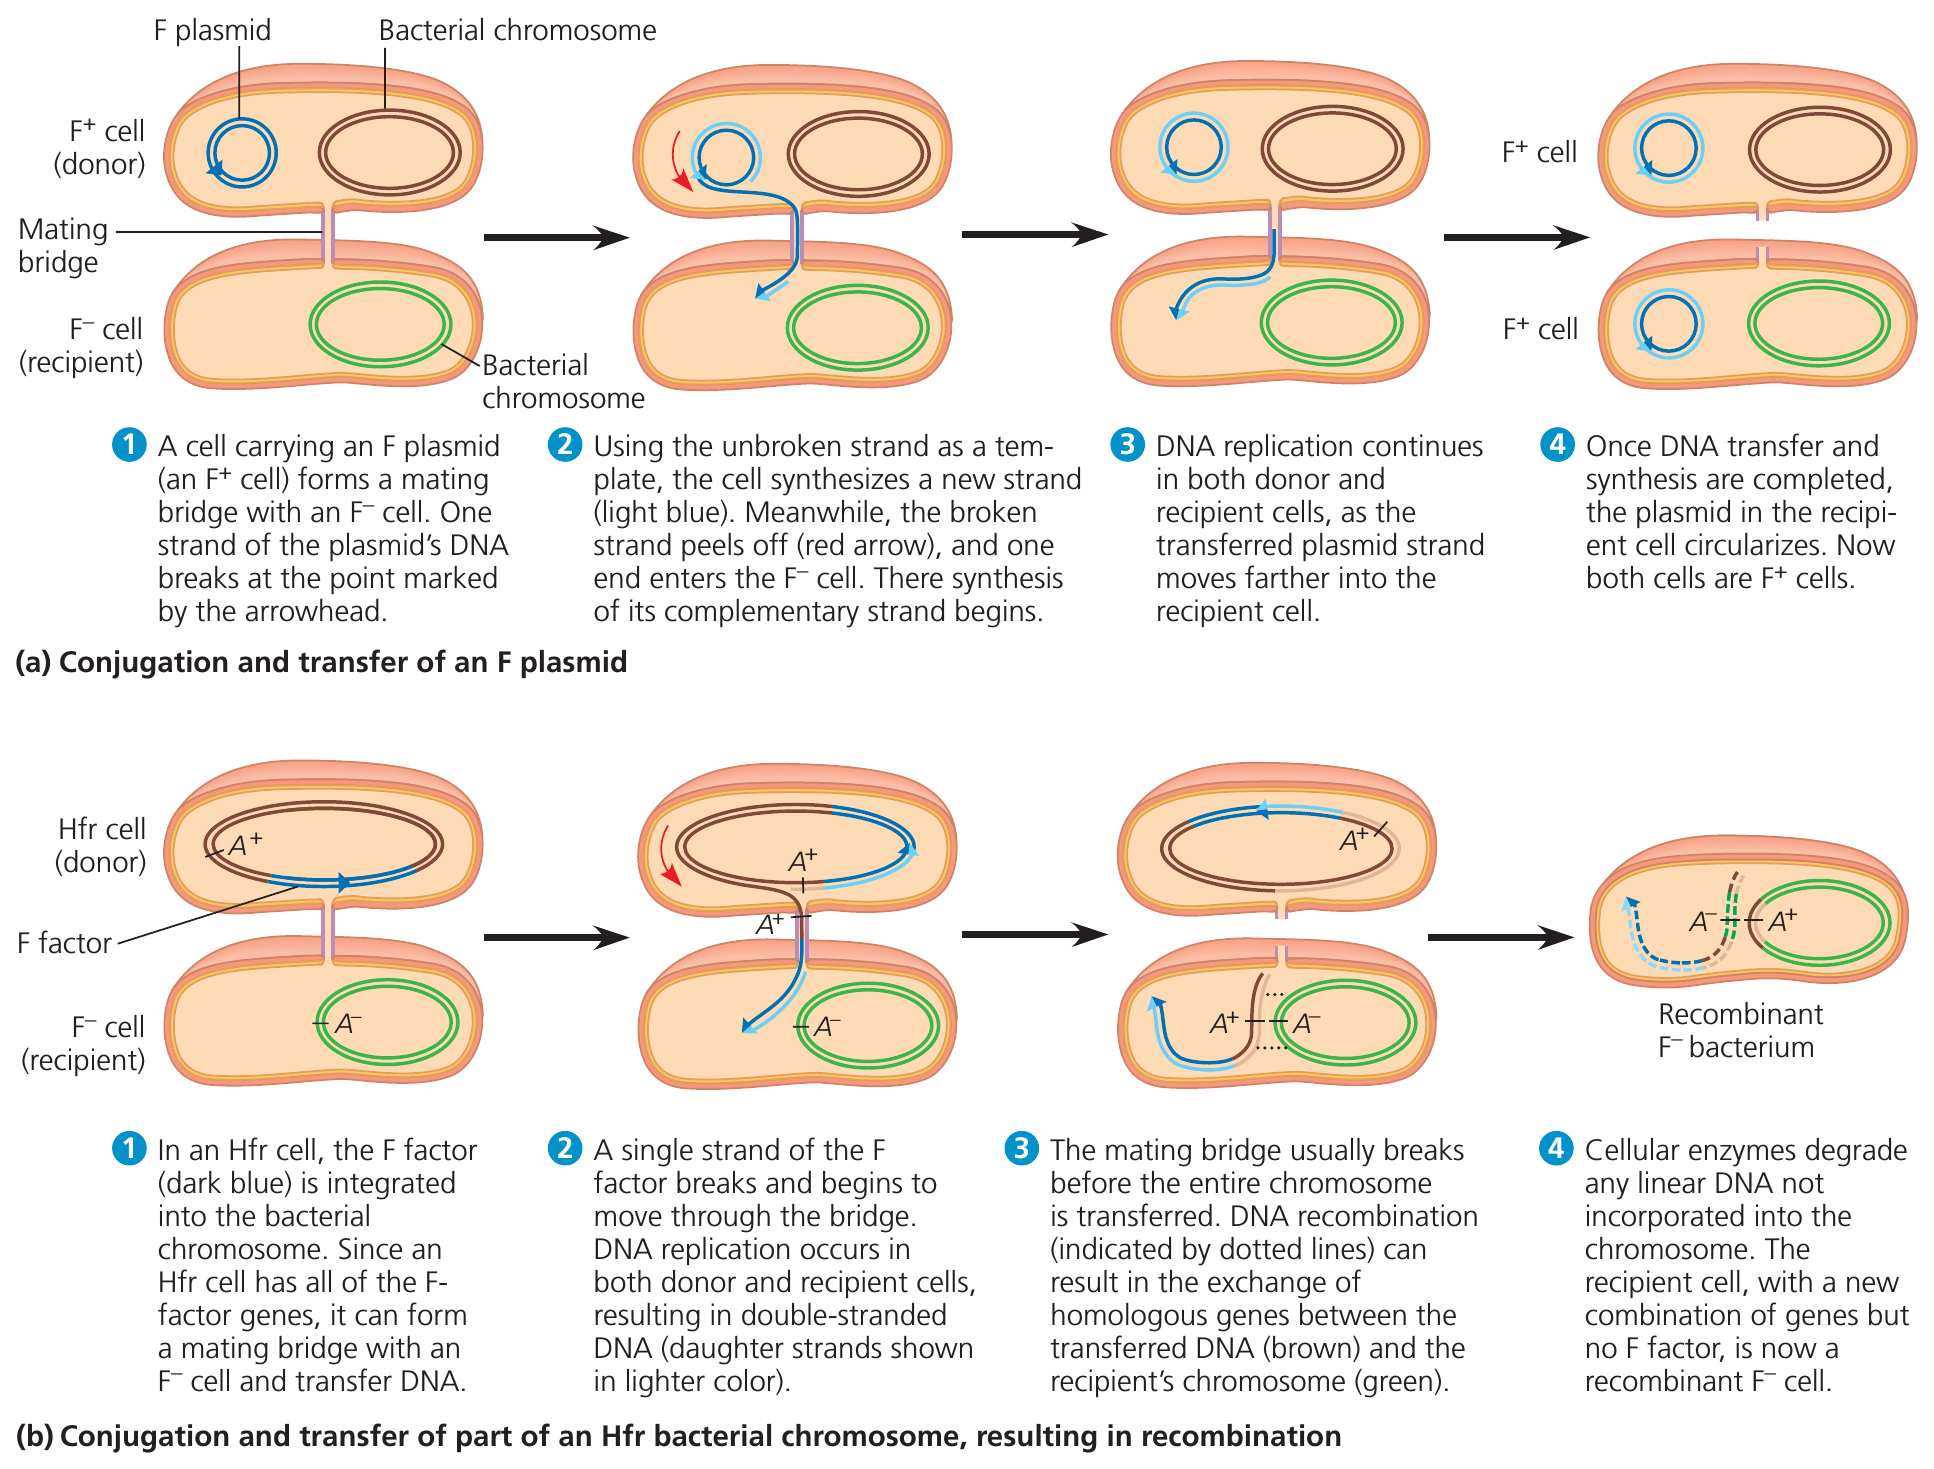
\includegraphics[width=0.5\linewidth]{./../images/bacterial_conjugation2} \caption{Conjugation and recombination in E. coli. The DNA replication that accompanies transfer of an F plasmid or part of an Hfr bacterial chromosome is called rolling circle replication. In effect, the intact circular parental DNA strand “rolls” as its other strand peels off and a new complementary strand is synthesized.}\label{fig:conjugation2}
\end{figure}

\end{frame}

\begin{frame}{Protoplast fusion}
\protect\hypertarget{protoplast-fusion}{}

\begin{itemize}
\tightlist
\item
  Mostly successful in eukaryotic cells.
\item
  The protoplasts (cells that have been stripped of their walls) must be
  prepared by various enzymatic or antibiotic treatments.
\item
  Fusion of cell membranes is aided by a high concentration of
  polyethylene glycol.
\item
  The resulting diploid cell usually segregates haploid offspring, many
  of which show extensive recombination of parental characters.
\end{itemize}

\end{frame}

\begin{frame}{Protoplast fusion}
\protect\hypertarget{protoplast-fusion-1}{}

\begin{itemize}
\tightlist
\item
  The diploid state can be stable over many generations, as evidenced by
  successful transformation of parental genes whose phenotype was not
  present in the diploid donor cell.
\item
  Successful fusions have been reported with \emph{Actinoplanes},
  \emph{Brevibacterium}, \emph{Bacillus}, \emph{Mycobacterium},
  \emph{Providencia}, \emph{Staphylococcus}, and \emph{Streptomyces}.
\end{itemize}

\end{frame}

\begin{frame}{Protoplast fusion}
\protect\hypertarget{protoplast-fusion-2}{}

\begin{figure}
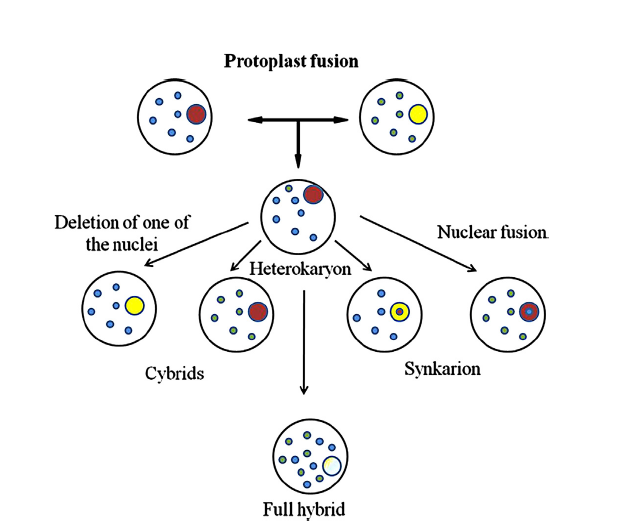
\includegraphics[width=0.3\linewidth]{./../images/protoplast_fusion} \caption{Formation of recombinants using protoplast fusion techniques}\label{fig:protoplast-fusion}
\end{figure}

\end{frame}

\begin{frame}{Electroporation}
\protect\hypertarget{electroporation}{}

\begin{itemize}
\tightlist
\item
  When a high voltage (as much as 2500 V) is passed from a capacitor
  through a solution containing living cells, significant damage occurs
  to cell membranes, and many cells die.
\item
  Among the survivors, however, are cells that developed small holes
  (pores) in their cell membranes as a result of the brief passage of
  current.
\item
  These pores are quickly sealed, but while they are open, solutes can
  pass into or out of the cytoplasm.
\item
  Plasmid DNA molecules can also enter a cell if the exterior
  concentration is sufficiently high.
\item
  This technique has been very successful with Gram-negative bacteria
  and somewhat less successful with Gram-positive bacteria.
\end{itemize}

\end{frame}

\begin{frame}{Bacteriophage genetic exchange}
\protect\hypertarget{bacteriophage-genetic-exchange}{}

\begin{itemize}
\tightlist
\item
  Viral genetics can be studied effectively by arranging the virus/cell
  ratio so that a cell is simultaneously infected by more than one virus
  particle.
\item
  Assuming that the two viruses are genetically distinguishable,
  selection is applied to prevent parent-type phage particles from
  successfully completing an infection.
\item
  Under these conditions, only cells in which phages carrying
  recombinant DNA have been produced yield progeny virus particles.
\item
  The resulting virions are tested for phenotype, and recombination
  frequency is calculated in the same manner as for bacteria.
\end{itemize}

\end{frame}

\end{document}
